\chapter{Love, Sex, and Pleasure}

This conversation continues the inquiry into transformation, attention, hurt, and relationship by turning to love. It is not a lecture with blackboard equations; its precision lies in distinctions. We therefore use a small amount of symbolic notation only as bookkeeping for the movement of the inquiry, not as a formal psychological theory. The source is J. Krishnamurti's dialogue with Dr. Alan W. Anderson, from material of the Krishnamurti Foundation Trust, curated for this course by LazyingArt LLC with Video2Book.

\section{The Word as a Mirror}

Anderson begins by carrying forward the previous conversation. They had been speaking about religion, not as belief or institution, but in relation to transformation, attention, and the whole history of hurt. At the end of that discussion they had touched love. The natural next move is to ask whether love can now be explored.

Krishnamurti first stops at the word \emph{explore}. The question is not casual. Are we exploring intellectually, as though love were a concept to be explained, or are we using the word as a mirror in which the human being observes himself? The distinction is the opening gate of the chapter.

We can write the movement schematically as
\begin{equation}
\text{word ``love''} \longrightarrow \text{mirror} \longrightarrow \text{observation of oneself}.
\end{equation}
This is not an equation in the usual sense. It is a compact way of preserving the order of the inquiry. The word is not to be treated as a label outside us; it reveals the movement of thought, desire, fear, memory, and image within us.

Krishnamurti adds that such exploration demands seriousness. Not solemnity, not intellectual heaviness, but the seriousness of a mind that is not trying to acquire love as an achievement. If the mind begins by asking how to become a successful lover, how to get love, how to possess the neighbor's love, it has already entered the field of desire and acquisition.

\section{The Corruption of the Word Love}

The lecture then moves through ordinary uses of the word. We say we love God, a wife, a husband, property, country, books, cinema, and pleasure. The word has become elastic enough to cover devotion, possession, amusement, appetite, and national identity. Krishnamurti's point is not linguistic neatness. If the word is confused, the inward observation is confused.

Modern education is brought into the inquiry at this point. Education has produced specialists: surgeons, physicians, technicians, scholars. But specialization by itself does not make the human mind serious. A clever specialist may still not know what it means to live. Anderson calls this figure a learned ignoramus, and Krishnamurti accepts the phrase because it names the split between knowledge and seriousness.

The chapter should therefore keep two tracks visible:
\begin{align}
\text{specialization} &\not\Longrightarrow \text{seriousness},\\
\text{knowledge} &\not\Longrightarrow \text{understanding of living}.
\end{align}
The inquiry into love begins only when this split is seen.

\section{Is Love Pleasure?}

Krishnamurti now places the central questions one after another. Is love pleasure? Is love the expression of desire? Is it sexual appetite fulfilled? Is it the pursuit of a desired end? Is it identification with family, woman, man, nation, or God? Is it something cultivated by practice?

The rhythm matters. He is not trying to define love immediately. He is clearing the field of false equations. The mind says ``love,'' but often means one of the following:
\begin{equation}
\text{love as means or pursuit}
\longrightarrow
\text{desire or pleasure}
\longrightarrow
\text{division}.
\end{equation}

\subsection{Question \& Answer}

\paragraph{Question.}
Can love be cultivated? If I have no love, can I think about it, work at it, practice it, and gradually produce it?

\paragraph{Answer.}
In the terms of this dialogue, that movement is already a denial of love. To cultivate love from lack is to make love into an object of achievement. The mind then stands in the field of desire: I do not have something, I want it, I shall acquire it, I shall become it. That is not love; it is becoming.

The same error appears in religious form. One says one loves God, but Krishnamurti asks what is actually happening. The pleasures of the world, sex, things, status, comfort, and consolation are transferred to a higher level and named God. The object is different, but the movement is still pleasure.

\section{Sex, Escape, and the Social Making of Pleasure}

The inquiry now moves from the general question of pleasure to the modern identification of love with sex. Krishnamurti is sharply struck by the phrase ``love-making,'' as though the physical act were love itself. He names cinema, books, pornography, advertising, stories, and the glamour industry as vehicles through which this identification has spread.

The next question is not moralistic. It is structural: why has sex become so enormous? The answer unfolds through the condition of the rest of life. If thought is second-hand, if the mind repeats Plato, Aristotle, Buddha, or any authority without freedom, it is intellectually crippled. If work is mechanical, if the office bullies, if the factory turns the human being into a function, then sex appears as the one place of relief.

The movement can be tracked as
\begin{align}
\text{second-hand thought} &\longrightarrow \text{intellectual unfreedom},\\
\text{mechanical social life} &\longrightarrow \text{felt imprisonment},\\
\text{romance and sentiment} &\longrightarrow \text{escape},\\
\text{escape through sex} &\longrightarrow \text{sex made enormous}.
\end{align}
This is the first worked reconstruction of the lecture's logic. It is not a biological theory of sex. It is the social and inward path by which pleasure becomes exaggerated when the rest of living has no freedom.

\begin{figure}
\centering
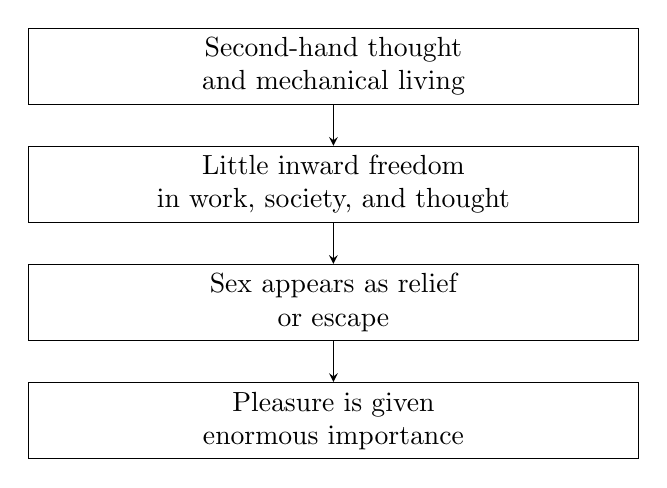
\begin{tikzpicture}[>=stealth]
\node[draw, align=center, text width=0.62\linewidth] (a) at (0,0) {Second-hand thought\\and mechanical living};
\node[draw, align=center, text width=0.62\linewidth] (b) at (0,-1.5) {Little inward freedom\\in work, society, and thought};
\node[draw, align=center, text width=0.62\linewidth] (c) at (0,-3.0) {Sex appears as relief\\or escape};
\node[draw, align=center, text width=0.62\linewidth] (d) at (0,-4.5) {Pleasure is given\\enormous importance};
\draw[->] (a) -- (b);
\draw[->] (b) -- (c);
\draw[->] (c) -- (d);
\end{tikzpicture}
\caption{A transcript-backed reconstruction of the movement by which sex becomes psychologically enormous.}
\end{figure}

Religion then enters with a contradiction. In one part of society sex is advertised and inflated; in another, it is denied, covered over, or condemned. Priests may preach celibacy while inwardly burning with desire. Krishnamurti does not accept either indulgence or repression as understanding.

\section{Celibacy and the Chaste Mind}

The conversation therefore asks what celibacy means. Is it the act, the vow, the outward abstention? Or is chastity a quality of mind?

\subsection{Question \& Answer}

\paragraph{Question.}
Is celibacy the outward act, or is chastity a condition of the mind?

\paragraph{Answer.}
The lecture rejects the merely outward answer. A mind may take a vow and still be filled with image, desire, fantasy, and conflict. Chastity, as Krishnamurti uses the word here, means a mind that is austere without severity, innocent because it is unhurt, and free of the picture of the woman, the man, or the act.

We can record the distinction in a compact table.

\begin{table}
\centering
\begin{tabular}{|p{0.42\linewidth}|p{0.42\linewidth}|}
\hline
\textbf{Outward celibacy} & \textbf{Chaste mind} \\
\hline
May be a vow, rule, or religious discipline. & Is a quality of mind, not merely an act. \\
\hline
May coexist with burning desire and image. & Has no inward image of possession, sex, or appetite. \\
\hline
Can become severe, proud, or repressive. & Is austere without brutality or severity. \\
\hline
Does not by itself end conflict. & Is innocent because it is not hurt. \\
\hline
\end{tabular}
\caption{The lecture's distinction between outward celibacy and inward chastity.}
\end{table}

This returns us to the previous inquiry into hurt. The chaste mind would not be hurt because it is not organized around an image. It has no picture of itself, of another, or of its own appetite. Anderson connects this with the old theological theme that the fall begins in imagination. Krishnamurti does not build a doctrine from that reference; he keeps the point direct: when image operates, conflict operates.

\section{Pleasure, Enjoyment, and Joy}

At the center of the lecture is a very exact distinction. Love cannot be understood until pleasure is understood. Pleasure is divisive; enjoyment is not divisive; joy is not divisive. But enjoyment can become pleasure when thought carries it over.

The temporal element is crucial. There is an immediate enjoyment: a meal, a sunset, a tree, a human face. If it ends there, it remains enjoyment. But thought remembers it, holds it, asks for its repetition tomorrow, and the carried-over movement becomes pleasure.

\begin{equation}
\text{enjoyment}
+
\text{thought carrying it over}
+
\text{demand for repetition}
\longrightarrow
\text{pleasure}.
\end{equation}

From there the lecture adds:
\begin{equation}
\text{pleasure} \longrightarrow \text{division}.
\end{equation}

\subsection{A Worked Example: How Enjoyment Becomes Pleasure}

Let us keep this as an explicit sequence.

\begin{enumerate}
\item There is an immediate perception: a beautiful sunset.
\item In that moment there is enjoyment.
\item Thought remembers the enjoyment.
\item Thought says, in effect, ``I want that again.''
\item The remembered enjoyment becomes a pursuit.
\item The pursuit is pleasure.
\item Because the pursuit is now mine, it divides.
\end{enumerate}

In this sense pleasure is not the same as enjoyment. Enjoyment is complete in the moment. Pleasure is enjoyment continued by thought.

\begin{figure}
\centering
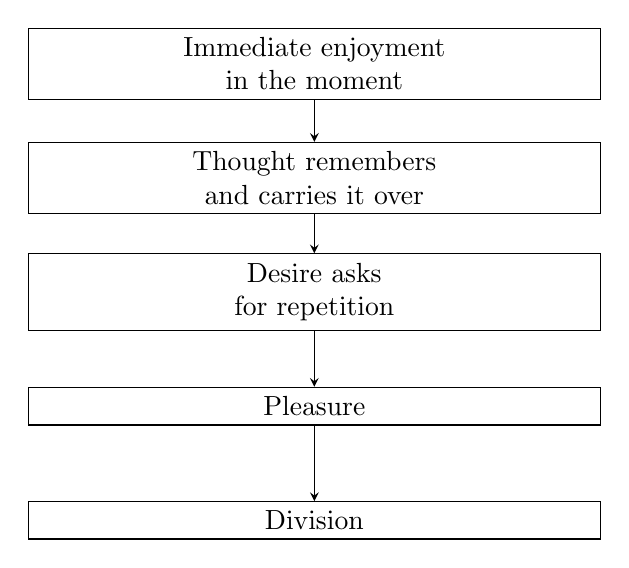
\begin{tikzpicture}[>=stealth]
\node[draw, align=center, text width=0.58\linewidth] (a) at (0,0) {Immediate enjoyment\\in the moment};
\node[draw, align=center, text width=0.58\linewidth] (b) at (0,-1.45) {Thought remembers\\and carries it over};
\node[draw, align=center, text width=0.58\linewidth] (c) at (0,-2.9) {Desire asks\\for repetition};
\node[draw, align=center, text width=0.58\linewidth] (d) at (0,-4.35) {Pleasure};
\node[draw, align=center, text width=0.58\linewidth] (e) at (0,-5.8) {Division};
\draw[->] (a) -- (b);
\draw[->] (b) -- (c);
\draw[->] (c) -- (d);
\draw[->] (d) -- (e);
\end{tikzpicture}
\caption{Enjoyment becomes pleasure when thought carries it over and seeks repetition.}
\end{figure}

Joy is treated still more delicately. Krishnamurti says that the moment joy is recognized, it is gone. Anderson brings in a remembered line from William Blake to point toward joy that is not held. The final notes should not turn this into literary commentary. The important distinction is that joy cannot be invited, possessed, or repeated by will.

\begin{table}
\centering
\begin{tabular}{|p{0.27\linewidth}|p{0.27\linewidth}|p{0.27\linewidth}|}
\hline
\textbf{Joy} & \textbf{Enjoyment} & \textbf{Pleasure} \\
\hline
Cannot be invited; recognition already alters it. & Immediate, complete when it ends in the moment. & Continuity of enjoyment through thought and repetition. \\
\hline
Not divisive. & Not divisive when it is not carried over. & Divisive because it becomes pursuit and possession. \\
\hline
Not produced by method. & Belongs to direct contact with what is. & Belongs to memory, desire, and becoming. \\
\hline
\end{tabular}
\caption{A compact reconstruction of the lecture's distinction between joy, enjoyment, and pleasure.}
\end{table}

\section{Love and Killing Cannot Be Joined}

The lecture then makes a severe turn. If pleasure is divisive, one must look at the forms division takes: pride, nationalism, power, ambition, religious ambition, and killing. A person may speak of love of country, but that love may be ready to kill. A priest may speak of God and yet be ambitious. A civilization may speak of morality and organize war.

The point can be stated as a proposition, with the caution that it is a faithful reconstruction of the dialogue, not a formal theorem.

\begin{proposition}
In this lecture, love cannot coexist with designed killing, ambition, and organized division.
\end{proposition}

\begin{proof}
Krishnamurti's reasoning proceeds by the movement of contradiction. Pleasure is divisive. Division appears as pride, nationalism, ambition, possession, and power. These movements sustain violence and organized killing. A mind participating inwardly in such division may use the word love, but the word has no substance in that field. Therefore the inquiry into love must also inquire into killing.
\end{proof}

The anecdote of the Buddhist couple in Ceylon tests this contradiction. They say they do not kill, yet they eat meat and solve the problem by changing butchers. The issue is not sectarian criticism; it is the human capacity to separate responsibility from action. Similarly, the lecture speaks of destroying the earth, wiping out species, killing animals for adornment or food, and preparing armies. Love is not being asked about in abstraction. It is being asked about in a world built on violence.

\subsection{Question \& Answer}

\paragraph{Question.}
If one is serious and one loves, does that mean one will never act when violence occurs?

\paragraph{Answer.}
No fixed answer is given in advance. Krishnamurti distinguishes designed killing from intelligent action in the moment. If someone is attacked, intelligence born of compassion acts then. But to prepare systems of killing, to organize enemies in advance, to build violence as policy, is not intelligence. It is design, fear, and division.

The contrast can be written as
\begin{align}
\text{compassion} &\longrightarrow \text{intelligence} \longrightarrow \text{action in the situation},\\
\text{fear and division} &\longrightarrow \text{designed killing} \longrightarrow \text{organized violence}.
\end{align}

\section{Education, Seeing, and Aloneness}

Anderson then brings the inquiry to education. A student comes and asks, ``What must I do?'' Krishnamurti sees the trap: the question often asks for a means. If I can be given a method, I can continue as I am and add the method. But in this inquiry the means is not separate from the end. Seeing danger is action.

The cleanest form of the distinction is:
\begin{align}
\text{seeing danger} &\longrightarrow \text{immediate action},\\
\text{not seeing danger} &\longrightarrow \text{continuity of thought}.
\end{align}

\subsection{Question \& Answer}

\paragraph{Question.}
What am I to do in this world?

\paragraph{Answer.}
Krishnamurti first reframes the question: what is my place in this world? The answer begins with the statement that the world is me. The corruption, war, superstition, killing, and lack of love are not merely outside. If I am that, I am in relationship to it as part of it. If I am not that, my relationship to it is of another order.

This leads into aloneness. Aloneness is not isolation, withdrawal, or an ivory tower. Isolation is produced by ambition, nationalism, family possession, fulfillment, and self-centered action. Aloneness comes when those movements are seen as false and negated without violence.

\begin{figure}
\centering
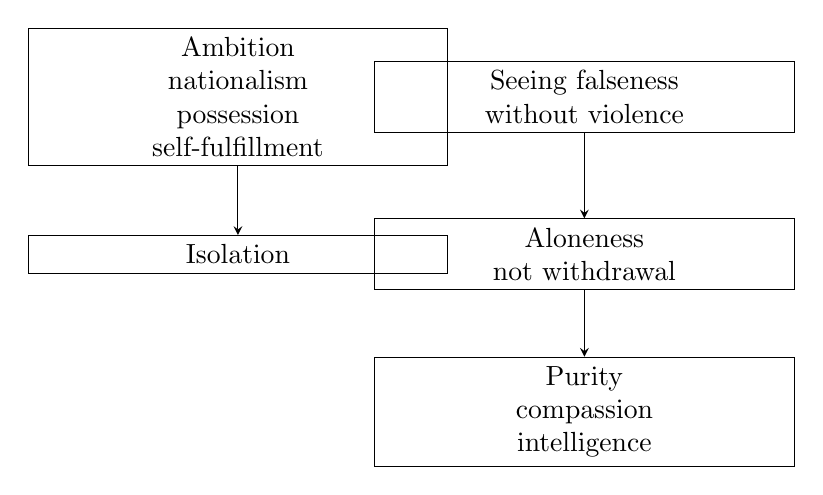
\begin{tikzpicture}[>=stealth]
\node[draw, align=center, text width=0.42\linewidth] (a) at (-2.2,0) {Ambition\\nationalism\\possession\\self-fulfillment};
\node[draw, align=center, text width=0.42\linewidth] (b) at (-2.2,-2.0) {Isolation};
\node[draw, align=center, text width=0.42\linewidth] (c) at (2.2,0) {Seeing falseness\\without violence};
\node[draw, align=center, text width=0.42\linewidth] (d) at (2.2,-2.0) {Aloneness\\not withdrawal};
\node[draw, align=center, text width=0.42\linewidth] (e) at (2.2,-4.0) {Purity\\compassion\\intelligence};
\draw[->] (a) -- (b);
\draw[->] (c) -- (d);
\draw[->] (d) -- (e);
\end{tikzpicture}
\caption{The lecture's distinction between isolating activity and aloneness.}
\end{figure}

Krishnamurti says that such aloneness is pure, not my purity or your purity, but purity. Anderson adds the image of fullness from Sanskrit. The important point is not a doctrine of solitude. It is the quality of a mind that has not withdrawn from the world but is no longer inwardly made of its corruption.

The final practical test concerns money entrusted to a friend who later denies receiving it. What is love there? It is not sentimental forgiveness that merely walks away. Love is intelligence, and intelligence is sensitivity to the situation. If recovery is possible, intelligence may act. If one has already decided what to do, or acts from hurt, the action is insensitive.

Thus the final chain is:
\begin{equation}
\text{love or compassion}
\longrightarrow
\text{intelligence}
\longrightarrow
\text{sensitivity to the situation}
\longrightarrow
\text{appropriate action}.
\end{equation}
This chain must remain flexible. The lecture refuses a precomputed answer. The situation, when met sensitively, tells the mind what action is.

\section{Summary}

The chapter's movement is one continuous inquiry. The word love is first made into a mirror. The corrupted uses of the word are exposed. Pleasure, desire, sex, cultivation, ambition, and religious projection are examined as substitutes for love. Sex becomes enormous because much of life is inwardly unfree; celibacy becomes false when it is only outward; chastity is a quality of mind without hurt and image.

The central distinction is that enjoyment becomes pleasure when thought carries it over and seeks repetition. Pleasure divides. That division shows itself not only in private desire but in nationalism, pride, ambition, and killing. Therefore the inquiry into love must include violence.

The close of the dialogue turns toward education, action, aloneness, compassion, and intelligence. Seeing danger is action; method-seeking is delay. Aloneness is not isolation, but the purity of a mind that has seen falseness and is no longer inwardly made of it. Love, at the end of this conversation, is not pleasure, not forgiveness as sentiment, not cultivation, and not possession. It is inseparable from intelligence and from sensitivity to what is actually taking place.